% Created 2023-10-28 sáb 21:55
% Intended LaTeX compiler: pdflatex
\documentclass[11pt]{article}
\usepackage[utf8]{inputenc}
\usepackage[T1]{fontenc}
\usepackage{graphicx}
\usepackage{longtable}
\usepackage{wrapfig}
\usepackage{rotating}
\usepackage[normalem]{ulem}
\usepackage{amsmath}
\usepackage{amssymb}
\usepackage{capt-of}
\usepackage{hyperref}
\usepackage{minted}
\usepackage[margin=0.5in]{geometry}
\author{Agustín Alejandro Mota Hinojosa}
\date{\today}
\title{3-4: Using Transaction Control Statements}
\hypersetup{
 pdfauthor={Agustín Alejandro Mota Hinojosa},
 pdftitle={3-4: Using Transaction Control Statements},
 pdfkeywords={},
 pdfsubject={},
 pdfcreator={Emacs 29.1 (Org mode 9.7)}, 
 pdflang={English}}
\begin{document}

\maketitle
\tableofcontents

\section{Vocabulary}
\label{sec:orgc77e431}
\begin{enumerate}
\item An inseparable list of database operations, which must be executed either in its entirety or not at all.

\textbf{Transaction}

\item Used for discarding any changes that were made to the database after the last COMMIT.

\textbf{Rollback}

\item Used toollbackn intermediate point in transaction processing.

\textbf{Savepoint}

\item Keyword used to signal the end of a PL/SQL block, not the end of a transaction.

\textbf{END}

\item Statement used to make database changes permanent.

\textbf{Commit}
\end{enumerate}
\section{Try It / Solve It}
\label{sec:orgc58bd9f}
\begin{enumerate}
\item How many transactions are shown in the following code? Explain your reasoning.
\begin{minted}[]{sql}
    begin
        insert into my_savings (account_id, amount) values (10377, 200);
        insert into my_checking (account_id, amount) values (10378, 100);
    end;
\end{minted}

\item Create the endangered species table by running the following statement in Application Express:
\begin{minted}[]{sql}
    create table endangered_species (
     (species_id number(4) constraint es_spec_pk primary key,
     common_name varchar2(30) constraint es_com_name_nn not null,
     scientific_name varchar2(30) constraint es_sci_name_nn not null));
\end{minted}

\begin{center}
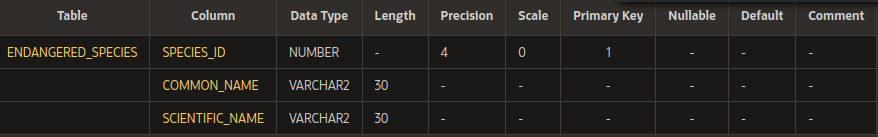
\includegraphics[width=.9\linewidth]{./resources/2023-10-28_21-47.png}
\end{center}

\item Examine the following block of code. If you were to run this block, what data do you think would be saved in the database?
\begin{minted}[]{sql}
    begin
        insert into endangered_species values (100, 'polar bear', 'ursus maritimus');
        savepoint sp_100;
        insert into endangered_species values (200, 'spotted owl', 'strix occidentalis');
        savepoint sp_200;
        insert into endangered_species values (300, 'asiatic black bear', 'ursus thibetanus');
        rollback to sp_100;
        commit;
    end;
\end{minted}

\texttt{100, 'Polar Bear','Ursus maritimus'}

\item Run the block above to test your theory. Confirm your projected data was added.

\begin{center}
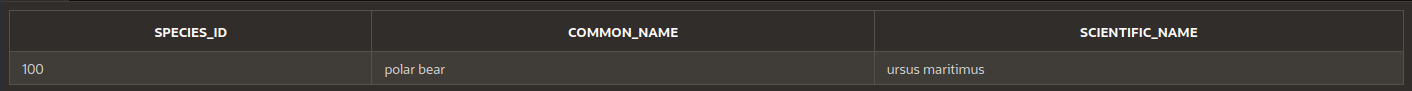
\includegraphics[width=.9\linewidth]{./resources/select_ensp.png}
\end{center}

\item Examine the following block. If you were to run this block, what data do you think would be saved in the database? Run the block to test your theory.
\begin{minted}[]{sql}
    begin
        insert into endangered_species values (400, 'blue gound beetle', 'carabus intricatus');
        savepoint sp_400;
        insert into endangered_species values (500, 'little spotted cat', 'leopardus tigrinus');
        rollback;
        insert into endangered_species values (600, 'veined tongue-fern', 'elaphoglossum nervosum');
        rollback to sp_400;
    end;
\end{minted}

No data will be saved.
\end{enumerate}
\end{document}